\documentclass[11pt]{article}
\usepackage[utf8]{inputenc}
\usepackage[T1]{fontenc}
\usepackage{amsmath}
\usepackage{amssymb} % Needed for \eth
\usepackage{graphicx}
\usepackage{geometry}
\usepackage{tikz}
\usepackage{pgfplots} % For plots
\usepackage{ulem}     % For underline, using normalem to avoid messing with \emph
\usepackage{tcolorbox} % For boxing equations
\usepackage{braket}    % For QM state notation if needed

\geometry{a4paper, margin=1in}
\usetikzlibrary{positioning, arrows.meta, shapes.geometric, patterns, calc} % Added calc library
\pgfplotsset{compat=1.18} % Use a recent PGFPlots version

% Custom commands (optional)
\newcommand{\avg}[1]{\overline{#1}}
\newcommand{\prob}[1]{P(#1)}
\newcommand{\ProbDens}[1]{\mathcal{P}(#1)} % Using script P for density
\newcommand{\vect}[1]{\vec{#1}}
\newcommand{\dd}[1]{\mathrm{d}#1} % Differential d
\newcommand{\pderiv}[2]{\frac{\partial #1}{\partial #2}}
\newcommand{\deriv}[2]{\frac{\mathrm{d} #1}{\mathrm{d} #2}}
\newcommand{\muState}{\mu\text{-state}} % Microstate
\newcommand{\OmegaE}{\Omega(E)}
\newcommand{\omegaE}{\omega(E)}
\newcommand{\PhiE}{\Phi(E)}
\newcommand{\deltaE}{\delta E}
\newcommand{\ethbar}{\text{\it{đ}}} % \eth symbol for inexact differential
\newcommand{\kb}{k_B} % Boltzmann constant
\newcommand{\gasR}{R} % Ideal gas constant
\newcommand{\partfn}{Z} % Partition function symbol
\newcommand{\grandpartfn}{\mathcal{Z}} % Grand partition function symbol
\newcommand{\lambdaT}{\lambda_{th}} % Thermal wavelength

% Define a tcolorbox style for boxed equations
\tcbuselibrary{skins}
\newtcolorbox{eqbox}[1][]{
  enhanced,
  colback=yellow!10!white,
  colframe=blue!75!black,
  boxrule=1pt,
  arc=3mm,
  #1
}

\title{Physics 415 - Lecture 23: Classical Limit, Equipartition Theorem}
\date{March 14, 2025}
\author{} % Author not specified

\begin{document}

\maketitle
\thispagestyle{empty}

\section*{Summary}

\begin{itemize}
    \item Canonical Ensemble (CE): Fixed $T, V, N$. $P_r = e^{-\beta E_r} / \partfn$, $\partfn = \sum_r e^{-\beta E_r}$ ($\beta=1/T$). $F = -T \ln \partfn$.
    \item Classical Partition Function ($N$ identical particles):
    \[ \partfn = \frac{1}{N!} \int \prod_{i=1}^N \frac{d^3 q_i d^3 p_i}{(2\pi\hbar)^3} e^{-\beta E(q,p)} \]
    \[ \partfn = \frac{1}{N!} \xi^N \int \prod_{i=1}^N \frac{d^3 q_i}{V} e^{-\beta U(q)} \]
    where $\xi = V / \lambdaT^3$ is related to the single-particle partition function, and $\lambdaT = h / \sqrt{2\pi m T}$ is the thermal de Broglie wavelength. $U(q)$ is potential energy (for ideal gas $U=0$).
\end{itemize}

\section*{Validity of the Classical Approach}

We have seen that a sensible partition function in classical statistical mechanics requires ingredients from Quantum Mechanics (QM): the phase space cell volume $(2\pi\hbar)^S$ and the $N!$ factor for indistinguishable particles.
Question: When is the classical approach valid? When must we resort to a full quantum treatment?

We can use the Heisenberg uncertainty relation $\Delta x \Delta p \sim \hbar$ to make some estimates of the "classical regime". (Note: This mixes classical and quantum reasoning, but gives the correct estimate. A more careful calculation uses a full QM treatment).
Estimate the typical momentum spread $\Delta p$: Average kinetic energy per DOF is $\sim T/2$, so $\avg{p^2 / (2m)} \sim T/2 \implies \avg{p^2} \sim mT$. Assume the spread is roughly the typical momentum magnitude: $\Delta p \sim \sqrt{\avg{p^2}} \sim \sqrt{mT}$.
This momentum uncertainty determines a minimum "size" or position uncertainty of the particle via QM:
\[ \Delta x \sim \frac{\hbar}{\Delta p} \sim \frac{\hbar}{\sqrt{mT}} \]
This leads to a characteristic length scale:
\[ \lambdaT \equiv \sqrt{\frac{2\pi\hbar^2}{mT}} = \frac{h}{\sqrt{2\pi m T}} \]
This is the \textbf{thermal de Broglie wavelength}, roughly the quantum "size" of a particle at temperature $T$. Note that $\lambdaT$ already appeared in the classical partition function:
\[ \xi = V \left( \frac{mT}{2\pi\hbar^2} \right)^{3/2} = V \left( \frac{h^2}{2\pi m T (2\pi\hbar)^2} \right)^{3/2} ? \]
Let's re-check $\xi = V (m / (2\pi\hbar^2\beta))^{3/2} = V (mT / (2\pi\hbar^2))^{3/2}$.
$\lambdaT^2 = h^2 / (2\pi m T) = (2\pi\hbar)^2 / (2\pi m T) = 2\pi\hbar^2 / (mT)$.
$mT / (2\pi\hbar^2) = 1/\lambdaT^2$.
So $\xi = V (1/\lambdaT^2)^{3/2} = V / \lambdaT^3$. Correct.
\[ Z = \frac{1}{N!} \left( \frac{V}{\lambdaT^3} \right)^N \int \prod \frac{d^3 q_i}{V} e^{-\beta U(q)} \quad (\text{Ideal gas } U=0 \implies \text{integral}=V^N) \]

It is reasonable to expect the classical treatment to be appropriate when the average distance 'a' between particles is much larger than their thermal wavelength $\lambdaT$:
\[ a \gg \lambdaT \quad (\text{Classical Regime}) \]
When $a \sim \lambdaT$, quantum mechanical effects (wave nature, interference, identity) become important.
We can rephrase this condition in terms of the particle density $n = N/V$. The average volume per particle is $1/n$, so $a \sim (1/n)^{1/3}$.
The condition becomes: $n^{-1/3} \gg \lambdaT$, or $1 \gg n^{1/3} \lambdaT$, or $1 \gg n \lambdaT^3$.
\[ n \lambdaT^3 \ll 1 \quad (\text{Classical Limit}) \]
The classical limit is reached if the density $n$ is sufficiently low or the temperature $T$ is sufficiently high ($\lambdaT \propto 1/\sqrt{T}$).

\textbf{Example 1:} He gas at $T=300$ K and $p=1$ atm.
$n \approx 3 \times 10^{19}$ cm$^{-3}$. Average distance $a = n^{-1/3} \approx 3 \times 10^{-7}$ cm.
Mass $m_{He} \approx 4 \times 1.67 \times 10^{-24}$ g.
$\lambdaT = h / \sqrt{2\pi m T} \approx 0.5 \times 10^{-8}$ cm.
Here $a \gg \lambdaT$. Classical treatment is valid.

\textbf{Example 2:} Electrons ($e^-$) in a typical metal.
$m_e \ll m_{He}$. Density $n \sim 10^{22} - 10^{23}$ cm$^{-3}$. $a \sim \text{few} \times 10^{-8}$ cm (lattice spacing).
$\lambdaT \sim 50 \times 10^{-8}$ cm at $T=300$ K.
Here $\lambdaT \gtrsim a$. Electrons in a metal form a highly quantum system even at room temperature.

\section*{Equipartition Theorem}

This is an important general result in classical statistical mechanics.
In many situations, the energy $E$ contains terms that are quadratic in momenta and/or coordinates.
\begin{itemize}
    \item Ideal gas kinetic energy: $K = \sum_{i=1}^N \frac{1}{2m} (p_{ix}^2 + p_{iy}^2 + p_{iz}^2)$. (Quadratic in momenta).
    \item Harmonic oscillator: $E = \frac{p^2}{2m} + \frac{1}{2} k q^2$. (Quadratic in $p$ and $q$).
\end{itemize}

\textbf{Theorem Statement:} In classical statistical mechanics, for a system in thermal equilibrium at temperature $T$, each degree of freedom (coordinate or momentum) that enters the Hamiltonian quadratically contributes, on average, $\frac{1}{2}T$ to the internal energy $\avg{E}$. (Using $T$ in energy units; otherwise $\frac{1}{2} \kb T$). It also contributes $\frac{1}{2}$ (or $\frac{1}{2}\kb$) to the heat capacity.

\textbf{Derivation:} Suppose the energy $E$ contains a term $\epsilon = \frac{1}{2} \kappa u^2$, where $u$ is some coordinate or momentum variable, and $E = \epsilon(u) + \tilde{E}(\text{other vars})$, where $\tilde{E}$ is independent of $u$.
The classical partition function $Z$ (ignoring $N!$ for simplicity here, as it won't affect averages) is:
\[ Z = \int \frac{dq dp}{(2\pi\hbar)^S} e^{-\beta E} = \left( \int' \frac{dq' dp'}{(2\pi\hbar)^{S-1}} e^{-\beta \tilde{E}} \right) \left( \int_{-\infty}^{\infty} \frac{du}{2\pi\hbar \text{ or } 1?} e^{-\beta \kappa u^2 / 2} \right) \]
% Need factor for du integration depending if q or p. Let's absorb into const.
\[ Z = \tilde{Z} \times \xi_u \]
where $\tilde{Z}$ involves integration over all variables except $u$, and $\xi_u$ is the factor from integrating over $u$:
\[ \xi_u = C' \int_{-\infty}^{\infty} du \, e^{-\beta \kappa u^2 / 2} = C' \sqrt{\frac{2\pi}{\beta \kappa}} \]
The average energy associated with the variable $u$ is $\avg{\epsilon} = \avg{\frac{1}{2}\kappa u^2}$. We can calculate this using the formula $\avg{E} = -\partial (\ln Z)/\partial \beta$.
The total average energy $\avg{E} = \avg{\tilde{E}} + \avg{\epsilon}$.
$\ln Z = \ln \tilde{Z} + \ln \xi_u$.
$\avg{E} = -\pderiv{}{\beta}(\ln \tilde{Z}) - \pderiv{}{\beta}(\ln \xi_u)$.
The first term is the average energy from all other degrees of freedom. The second term is the contribution from $u$:
\[ \avg{\epsilon} = -\pderiv{}{\beta}(\ln \xi_u) = -\pderiv{}{\beta} (\ln C' + \ln \sqrt{2\pi/(\beta\kappa)}) = -\pderiv{}{\beta} (\text{const} - \frac{1}{2}\ln \beta) \]
\[ \avg{\epsilon} = - (-\frac{1}{2} \frac{1}{\beta}) = \frac{1}{2\beta} = \frac{1}{2} T \]
So, each quadratic term $\frac{1}{2}\kappa u^2$ contributes $\frac{1}{2}T$ to the average energy.
The contribution to the heat capacity is $C_u = \partial \avg{\epsilon} / \partial T = \partial (\frac{1}{2}T)/\partial T = 1/2$. (Or $\kb/2$).

\textbf{Note:} This theorem is only true in classical statistical mechanics.

\subsection*{Simple Applications}

\begin{itemize}
    \item Single molecule (or atom) in gas at $T$: Translational kinetic energy $K = \frac{1}{2m}(p_x^2 + p_y^2 + p_z^2)$. Three quadratic terms.
    Contribution to average energy $= 3 \times (\frac{1}{2}T) = \frac{3}{2}T$.
    \item Monatomic ideal gas (N particles): $E = \sum_{i=1}^N K_i$. Total $3N$ quadratic terms.
    $\avg{E} = 3N \times (\frac{1}{2}T) = \frac{3}{2} NT$. $\checkmark$
    \item Classical 1D Harmonic Oscillator: $E = \frac{p^2}{2m} + \frac{1}{2} k q^2$. Two quadratic terms.
    $\avg{E} = 2 \times (\frac{1}{2}T) = T$.
    Note that the average kinetic energy $\avg{K} = \avg{p^2/(2m)} = T/2$ and average potential energy $\avg{U} = \avg{kq^2/2} = T/2$. Thus $\avg{K} = \avg{U} = \avg{E}/2$.
\end{itemize}

\subsection*{Quantum Harmonic Oscillator Revisited}

It is interesting to see how the harmonic oscillator result is modified in QM.
Energy levels: $E_n = (n+1/2)\hbar\omega$, $n=0, 1, 2, \dots$.
Partition function: $Z = \sum_{n=0}^\infty e^{-\beta E_n} = \sum_{n=0}^\infty e^{-\beta(n+1/2)\hbar\omega} = e^{-\beta\hbar\omega/2} \sum_{n=0}^\infty (e^{-\beta\hbar\omega})^n$.
This is a geometric series $\sum_{n=0}^\infty x^n = 1/(1-x)$ with $x=e^{-\beta\hbar\omega}$.
\[ Z = \frac{e^{-\beta\hbar\omega/2}}{1 - e^{-\beta\hbar\omega}} \]
Average energy: $\avg{E} = -\pderiv{}{\beta}(\ln Z)$.
$\ln Z = -\frac{\beta\hbar\omega}{2} - \ln(1 - e^{-\beta\hbar\omega})$.
\[ \avg{E} = - \left[ -\frac{\hbar\omega}{2} - \frac{1}{1 - e^{-\beta\hbar\omega}} (-e^{-\beta\hbar\omega}) (-\hbar\omega) \right] \]
\[ \avg{E} = \frac{\hbar\omega}{2} + \frac{\hbar\omega e^{-\beta\hbar\omega}}{1 - e^{-\beta\hbar\omega}} = \frac{\hbar\omega}{2} + \frac{\hbar\omega}{e^{\beta\hbar\omega} - 1} \]
\[ \avg{E} = \hbar\omega \left( \frac{1}{2} + \frac{1}{e^{\hbar\omega/T} - 1} \right) \]
(Includes zero-point energy $\hbar\omega/2$).

\textbf{Limits:}
\begin{itemize}
    \item High T limit ($T \gg \hbar\omega \implies \beta\hbar\omega \ll 1$): Let $x = \beta\hbar\omega = \hbar\omega/T$. $e^x \approx 1+x$.
    $\avg{E} \approx \hbar\omega (\frac{1}{2} + \frac{1}{(1+x)-1}) = \hbar\omega (\frac{1}{2} + \frac{1}{x}) = \hbar\omega (\frac{1}{2} + \frac{T}{\hbar\omega}) = \frac{\hbar\omega}{2} + T$.
    Excluding the zero-point energy, $\avg{E} - E_0 \approx T$. This recovers the classical equipartition result ($\avg{E}_{classical}=T$).
    \item Low T limit ($T \ll \hbar\omega \implies \beta\hbar\omega \gg 1$): $e^{\beta\hbar\omega} \gg 1$.
    $\avg{E} \approx \hbar\omega (\frac{1}{2} + e^{-\beta\hbar\omega}) = \frac{\hbar\omega}{2} + \hbar\omega e^{-\hbar\omega/T}$.
    As $T \to 0$, $\avg{E} \to \hbar\omega/2$ (ground state energy).
\end{itemize}

Sketch of $\avg{E}$ vs $T$:
\begin{center}
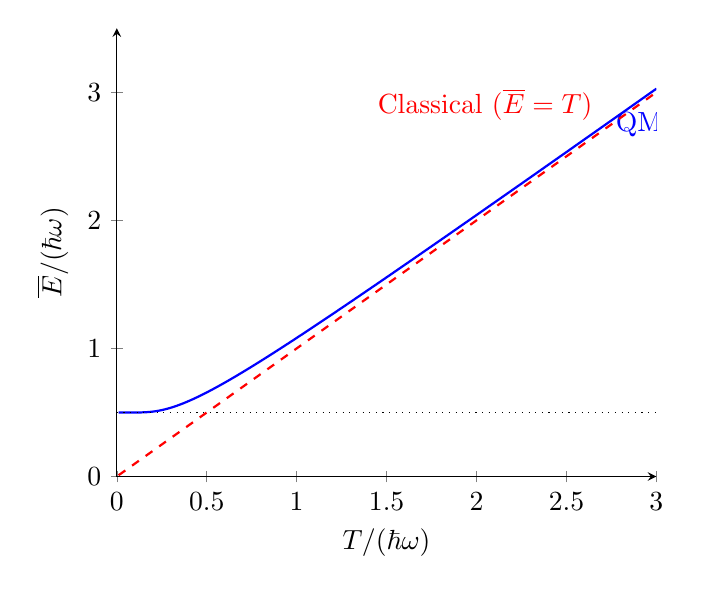
\begin{tikzpicture}
\begin{axis}[
    xlabel={$T / (\hbar\omega)$}, ylabel={$\avg{E} / (\hbar\omega)$},
    xmin=0, xmax=3, ymin=0, ymax=3.5,
    axis lines=left,
    legend pos=north west
]
\addplot [domain=0.01:3, samples=100, smooth, thick, blue] {0.5 + 1/(exp(1/x)-1)} node[pos=0.9, anchor=west] {QM};
\addplot [domain=0.01:3, samples=50, dashed, thick, red] {x} node[pos=0.9, anchor=south east] {Classical ($\avg{E}=T$)};
\draw [dotted] (axis cs:0, 0.5) -- (axis cs:3, 0.5) node[pos=0, left] {$1/2$}; % Zero point energy
\end{axis}
\end{tikzpicture}
\end{center}

Heat Capacity $C = \partial \avg{E} / \partial T$.
\[ C = \pderiv{}{T} \left[ \hbar\omega \left( \frac{1}{2} + \frac{1}{e^{\hbar\omega/T} - 1} \right) \right] = \hbar\omega \frac{-1}{(e^{\hbar\omega/T} - 1)^2} \left( e^{\hbar\omega/T} \right) \left( -\frac{\hbar\omega}{T^2} \right) \]
\[ C = \left( \frac{\hbar\omega}{T} \right)^2 \frac{e^{\hbar\omega/T}}{(e^{\hbar\omega/T} - 1)^2} \]
(Using $T$ in energy units, so $C$ is dimensionless, equivalent to $C/\kb$).

\textbf{Limits:}
\begin{itemize}
    \item High T limit ($x = \hbar\omega/T \ll 1$): $e^x \approx 1+x$. $C \approx x^2 \frac{1+x}{((1+x)-1)^2} = x^2 \frac{1+x}{x^2} \approx 1$. Agrees with classical $C=1$ (or $\kb$).
    \item Low T limit ($x = \hbar\omega/T \gg 1$): $e^x \gg 1$. $C \approx x^2 \frac{e^x}{(e^x)^2} = x^2 e^{-x} = (\frac{\hbar\omega}{T})^2 e^{-\hbar\omega/T}$. Goes to 0 exponentially as $T \to 0$.
\end{itemize}

Sketch of $C$ vs $T$:
\begin{center}
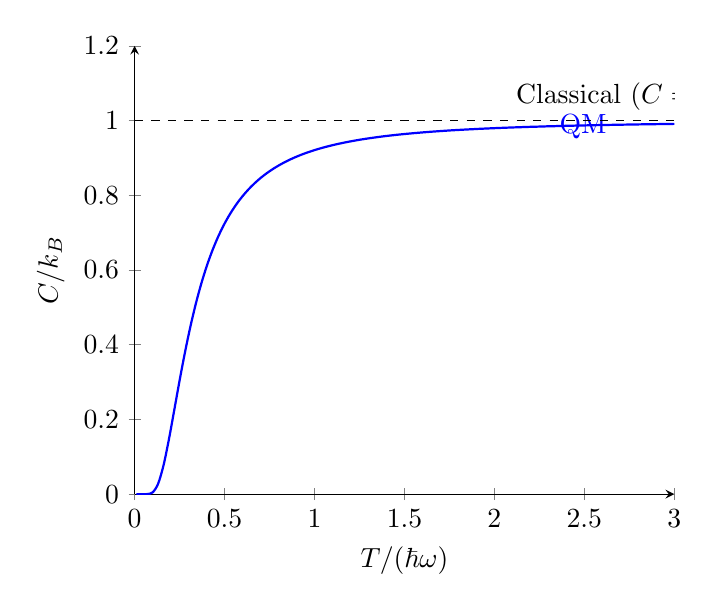
\begin{tikzpicture}
\begin{axis}[
    xlabel={$T / (\hbar\omega)$}, ylabel={$C / \kb$},
    xmin=0, xmax=3, ymin=0, ymax=1.2,
    axis lines=left,
    legend pos=south east
]
\addplot [domain=0.01:3, samples=100, smooth, thick, blue] {(1/x)^2 * exp(1/x) / (exp(1/x)-1)^2} node[pos=0.8, anchor=west] {QM};
\draw [dashed] (axis cs:0, 1) -- (axis cs:3, 1) node[pos=0.9, anchor=south] {Classical ($C=1$)};
\end{axis}
\end{tikzpicture}
\end{center}
Quantized energy levels lead to a dramatic reduction ("freezing out") of the heat capacity at low temperatures ($T \ll \hbar\omega$).

\end{document}